%%%%%%%%% wenn mehrere Anhänge vorhanden %%%%%%%%%
\begin{appendices}
    \chapter{Boxplot Deutscher Aggressionsfragebogen}            \label{Boxplot_AggroFB}
    %\addcontentsline{toc}{chapter}{A}
    \noindent \textit{Boxplot zur Erfassung der Ausreißer des Deutschen Aggressionsfragebogens}

    \begin{figure}[htb!]
        \centering
            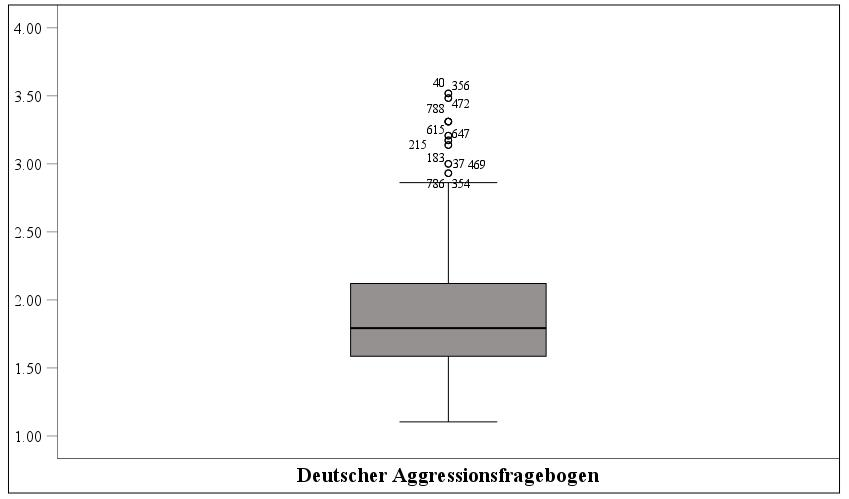
\includegraphics[width=\textwidth]{Boxplot AggroFB.jpg}
            %\caption[Linearer Zusammenhang des Deutschen Aggressionsfragebogens und des DVMAS]{Linearer Zusammenhang des Deutschen Aggressionsfragebogens und des DVMAS}

    \end{figure}
    
    

    %%%%%%%%%%%%%%%%%%%%%%%%%%%%%%%%%%%%%%%%%%%%

    \chapter{Boxplot DVMAS}            \label{Boxplot_DVMAS}
    %\addcontentsline{toc}{chapter}{B}
    \noindent \textit{Boxplot zur Erfassung der Ausreißer des DVMAS}

    \begin{figure}[htb!]
        \centering
            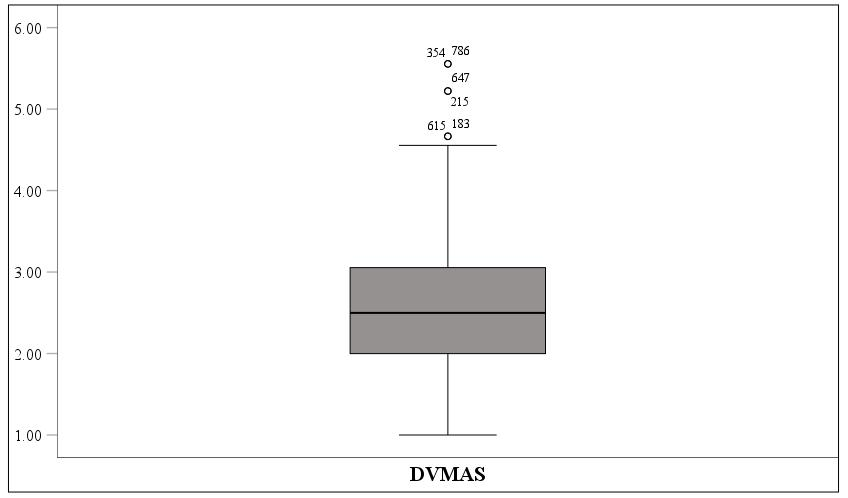
\includegraphics[width=\textwidth]{Boxplot DVMAS.jpg}
            %\caption[Linearer Zusammenhang des Deutschen Aggressionsfragebogens und des DVMAS]{Linearer Zusammenhang des Deutschen Aggressionsfragebogens und des DVMAS}

    \end{figure}
    
    

%%%%%%%%%%%%%%%%%%%%%%%%%%%%%%%%%%%%%%%%%%%%

\chapter{Linearität Deutscher Aggressionsfragebogen und DVMAS} \label{Linearitat_AggroFB_DVMAS}
%\addcontentsline{toc}{chapter}{C}
\noindent \textit{Linearer Zusammenhang des Deutschen Aggressionsfragebogens und des DVMAS}

\begin{figure}[htb!]
    \centering
        \includegraphics[width=\textwidth]{Linearität AggroFB-DVMAS.jpg}
        %\caption[Linearer Zusammenhang des Deutschen Aggressionsfragebogens und des DVMAS]{Linearer Zusammenhang des Deutschen Aggressionsfragebogens und des DVMAS}
        
\end{figure}
    
    

%%%%%%%%%%%%%%%%%%%%%%%%%%%%%%%%%%%%%%%%%%%%

    \chapter{Boxplot Aggression$-$Subskala physische Aggression}            \label{Boxplot_phAggro}
    %\addcontentsline{toc}{chapter}{D}
    \noindent \textit{Boxplot zur Erfassung der Ausreißer der Aggression$-$Subskala physische Aggression}

    \begin{figure}[htb!]
        \centering
            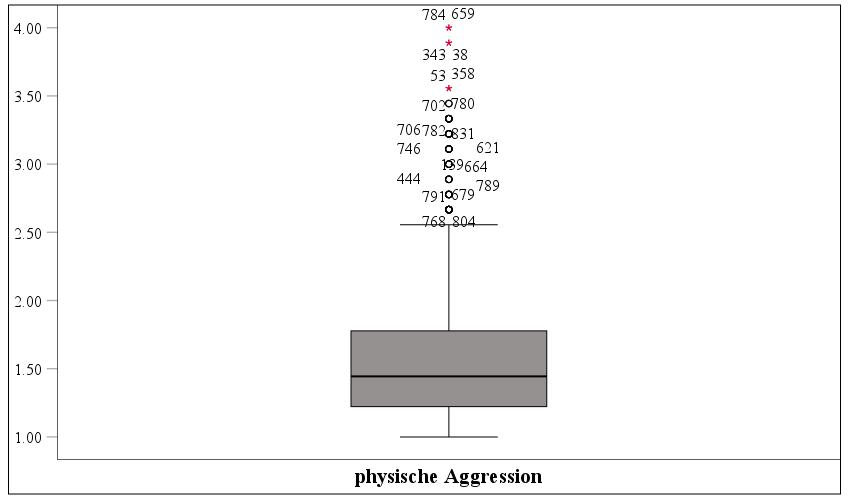
\includegraphics[width=\textwidth]{Boxplot ph_aggro.jpg}
            %\caption[Linearer Zusammenhang des Deutschen Aggressionsfragebogens und des DVMAS]{Linearer Zusammenhang des Deutschen Aggressionsfragebogens und des DVMAS}

    \end{figure}
    
    

%%%%%%%%%%%%%%%%%%%%%%%%%%%%%%%%%%%%%%%%%%%%

    \chapter{Online$-$Fragebogen}  \label{Fragebogen}
    %\addcontentsline{toc}{chapter}{E}
    \noindent \textit{Bildaufnahmen des Online$-$Fragbogens}

    \begin{figure}[htb!]
        \centering
            
\includegraphics[width=\textwidth]{Seite 1.png}
            \caption[]{Seite 1 des Online$-$Fragebogens}
    \end{figure}

    \newpage
    \begin{figure}[htb!]
        \centering
            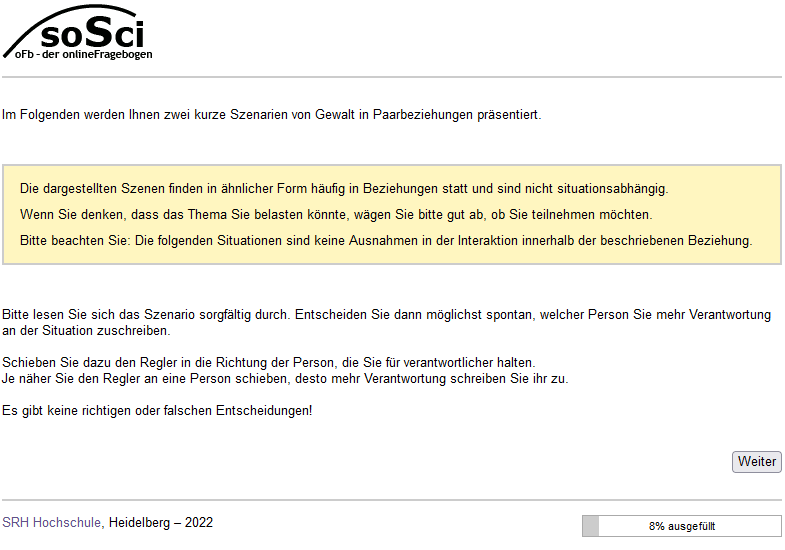
\includegraphics[width=\textwidth]{Seite 2.png}
            \caption[]{Seite 2 des Online$-$Fragebogens}
    \end{figure}

    \begin{figure}[htb!]
        \centering
            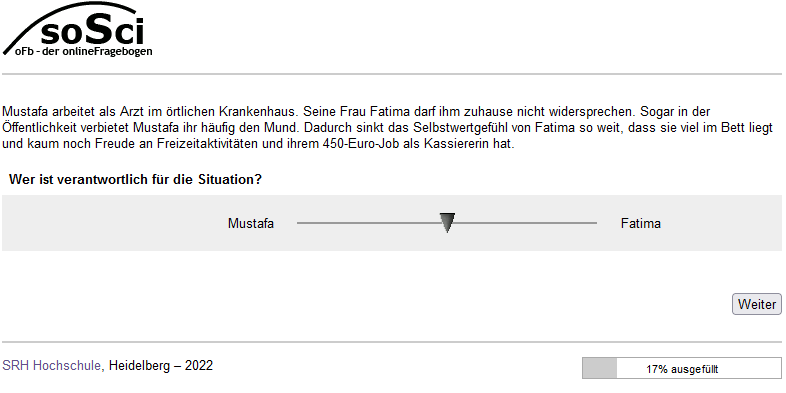
\includegraphics[width=\textwidth]{Seite 3.png}
            \caption[]{Seite 3 des Online$-$Fragebogens}
    \end{figure}
    
    \newpage
    \begin{figure}[htb!]
        \centering
            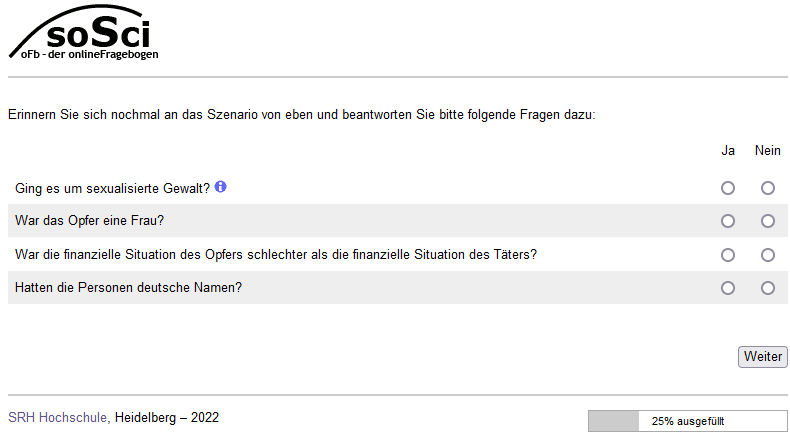
\includegraphics[width=\textwidth]{Seite 4.png}
            \caption[]{Seite 4 des Online$-$Fragebogens}
    \end{figure}
    
    \begin{figure}[htb!]
        \centering
            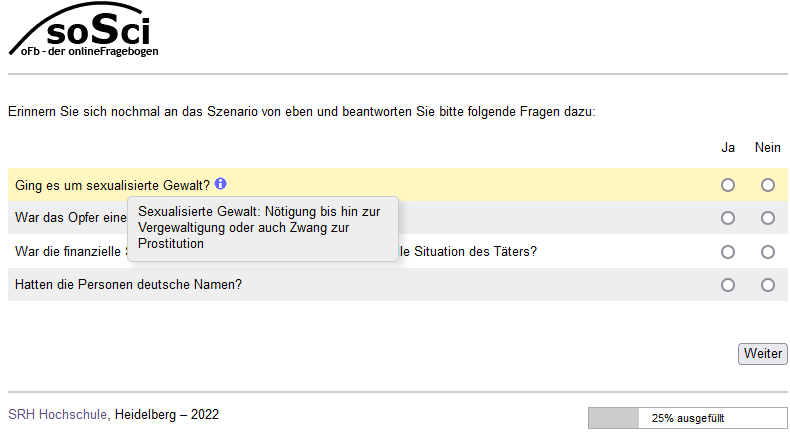
\includegraphics[width=\textwidth]{Seite 4 mit Infobox.png}
            \caption[]{Seite 4 des Online$-$Fragebogens mit Infobox}
    \end{figure}
    
    \newpage
    \begin{figure}[htb!]
        \centering
            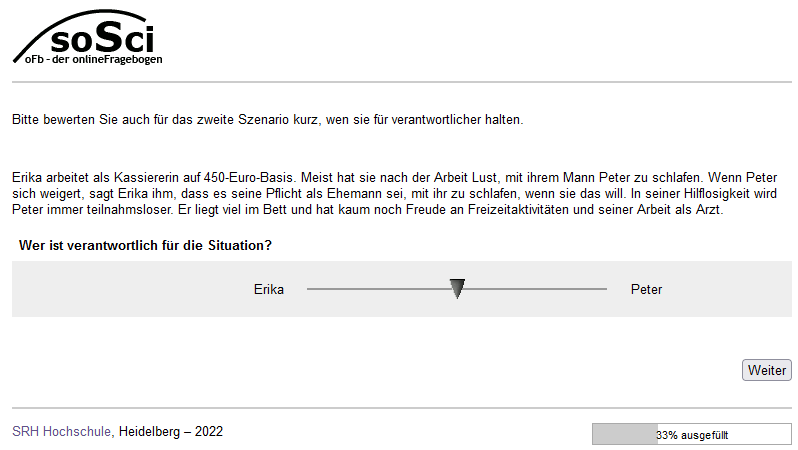
\includegraphics[width=\textwidth]{Seite 5.png}
            \caption[]{Seite 5 des Online$-$Fragebogens}
    \end{figure}
    
    \begin{figure}[htb!]
        \centering
            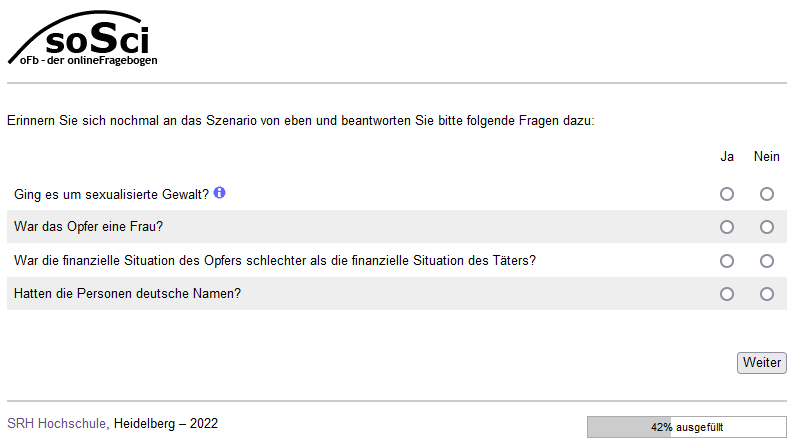
\includegraphics[width=\textwidth]{Seite 6.png}
            \caption[]{Seite 6 des Online$-$Fragebogens}
    \end{figure}
    
    \newpage
    \begin{figure}[htb!]
        \centering
            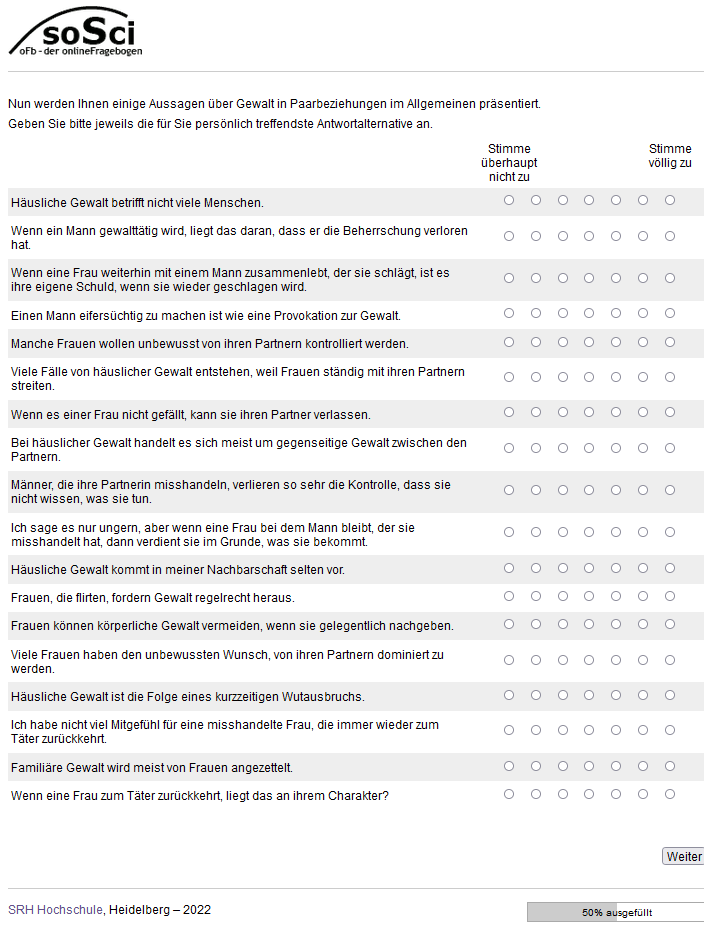
\includegraphics[width=\textwidth]{Seite 7.png}
            \caption[]{Seite 7 des Online$-$Fragebogens (deutsche Übersetzung des englischen DVMAS nach \textcite{Peters2003})}
    \end{figure}
    
    \newpage
    \begin{figure}[htb!]
        \centering
            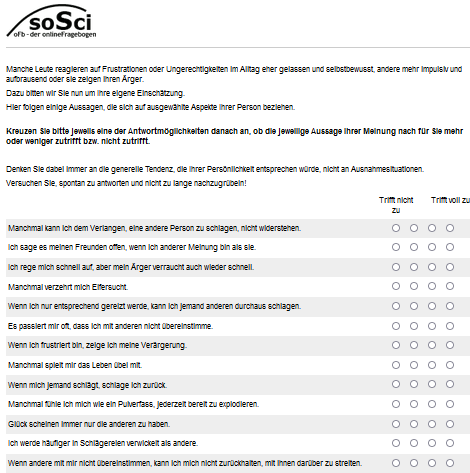
\includegraphics[width=\textwidth]{Seite 8_1.png}
            \caption[]{Erste Hälfte von Seite 8 des Online$-$Fragebogens des Deutschen Aggressionsfragebogens \parencite{Aggressionsfragebogen}}
    \end{figure}
    
    \newpage
    \begin{figure}[htb!]
        \centering
            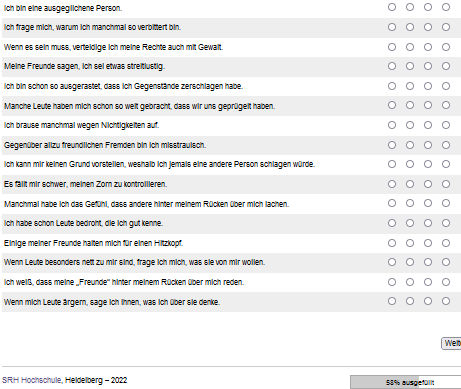
\includegraphics[width=\textwidth]{Seite 8_2.png}
            \caption[]{Zweite Hälfte von Seite 8 des Online$-$Fragebogens des Deutschen Aggressionsfragebogens \parencite{Aggressionsfragebogen}}
    \end{figure}
    
    \newpage
    \begin{figure}[htb!]
        \centering
            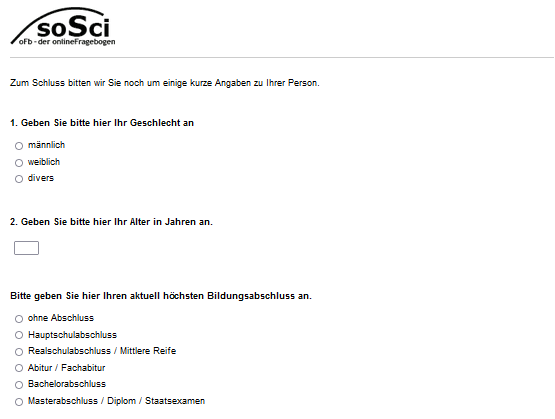
\includegraphics[width=\textwidth]{Seite 9_1.png}
            \caption[]{Erste Hälfte von Seite 9 des Online$-$Fragebogens}
    \end{figure}
    
    \newpage
    \begin{figure}[htb!]
        \centering
            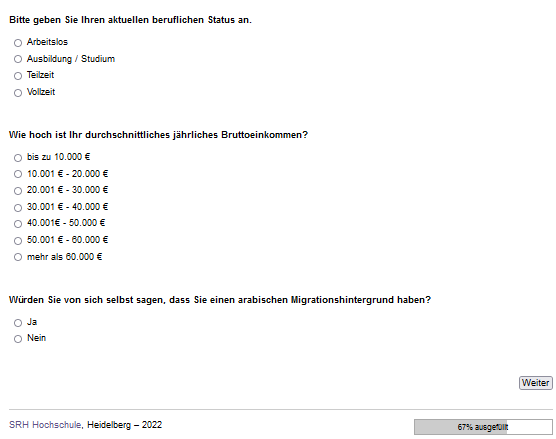
\includegraphics[width=\textwidth]{Seite 9_2.png}
            \caption[]{Zweite Hälfte von Seite 9 des Online$-$Fragebogens}
    \end{figure}
    
    \begin{figure}[htb!]
        \centering
            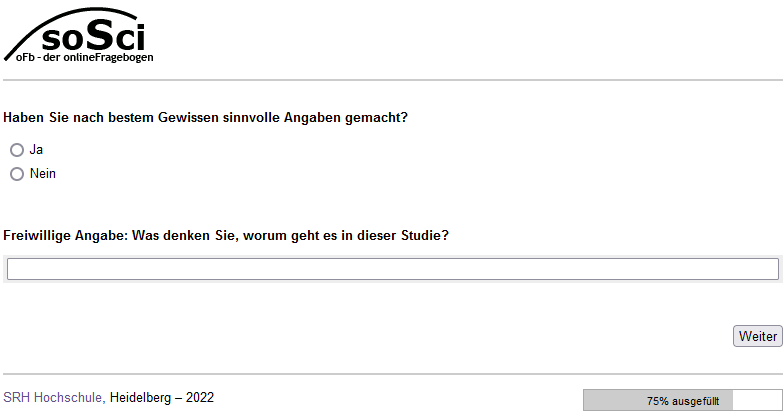
\includegraphics[width=\textwidth]{Seite 10.png}
            \caption[]{Seite 10 des Online$-$Fragebogens}
    \end{figure}
    
    \newpage
    \begin{figure}[htb!]
        \centering
            
\includegraphics[width=\textwidth]{Seite 11.png}
            \caption[]{Seite 11 des Online$-$Fragebogens}
    \end{figure}
    
    \begin{figure}[htb!]
        \centering
            
\includegraphics[width=\textwidth]{Seite 12.png}
            \caption[]{Seite 12 des Online$-$Fragebogens}
    \end{figure}


    
    

%%%%%%%%%%%%%%%%%%%%%%%%%%%%%%%%%%%%%%%%%%%%
\end{appendices}







%%%%%%%%% wenn mehrere Anhänge vorhanden %%%%%%%%%



%%%%%%%%% wenn nur 1 Anhang vorhanden %%%%%%%%%
%\chapter*{Anhang}
%\addcontentsline{toc}{chapter}{Anhang}
%\noindent \textit{Titel des Anhangs}

%Inhalt
%%%%%%%%% wenn nur 1 Anhang vorhanden %%%%%%%%%